\documentclass[a4paper, 12pt]{article}

\usepackage{arxiv}

\usepackage[T2A]{fontenc}
\usepackage[utf8]{inputenc}
\usepackage[english, russian]{babel}
% \usepackage{cmap}
\usepackage{url}
\usepackage{booktabs}
\usepackage{nicefrac}
\usepackage{microtype}
\usepackage{lipsum}
\usepackage{graphicx}
\usepackage{subfig}
\usepackage[square,sort,comma,numbers]{natbib}
\usepackage{doi}
\usepackage{multicol}
\usepackage{multirow}
\usepackage{tabularx}

\usepackage{tikz}
\usetikzlibrary{matrix}

% Algorithms
\usepackage{algpseudocode}
\usepackage{algorithm}

%% Шрифты
\usepackage{euscript} % Шрифт Евклид
\usepackage{mathrsfs} % Красивый матшрифт
\usepackage{extsizes} % Возможность сделать 14-й шрифт

\usepackage{makecell} % diaghead in a table
\usepackage{amsmath,amsfonts,amssymb,amsthm,mathtools,dsfont}
\usepackage{icomma}

\newcommand{\bz}{\mathbf{z}}
\newcommand{\bff}{\mathbf{f}}
\newcommand{\bx}{\mathbf{x}}
\newcommand{\by}{\mathbf{y}}
\newcommand{\bv}{\mathbf{v}}
\newcommand{\bw}{\mathbf{w}}
\newcommand{\ba}{\mathbf{a}}
\newcommand{\bb}{\mathbf{b}}
\newcommand{\bp}{\mathbf{p}}
\newcommand{\bq}{\mathbf{q}}
\newcommand{\bt}{\mathbf{t}}
\newcommand{\bg}{\mathbf{g}}
\newcommand{\bu}{\mathbf{u}}
\newcommand{\bT}{\mathbf{T}}
\newcommand{\bX}{\mathbf{X}}
\newcommand{\bZ}{\mathbf{Z}}
\newcommand{\bS}{\mathbf{S}}
\newcommand{\bH}{\mathbf{H}}
\newcommand{\bW}{\mathbf{W}}
\newcommand{\bM}{\mathbf{M}}
\newcommand{\bY}{\mathbf{Y}}
\newcommand{\bU}{\mathbf{U}}
\newcommand{\bQ}{\mathbf{Q}}
\newcommand{\bP}{\mathbf{P}}
\newcommand{\bA}{\mathbf{A}}
\newcommand{\bB}{\mathbf{B}}
\newcommand{\bC}{\mathbf{C}}
\newcommand{\bE}{\mathbf{E}}
\newcommand{\bF}{\mathbf{F}}
\newcommand{\bomega}{\boldsymbol{\omega}}
\newcommand{\btheta}{\boldsymbol{\theta}}
\newcommand{\bgamma}{\boldsymbol{\gamma}}
\newcommand{\bdelta}{\boldsymbol{\delta}}
\newcommand{\bPsi}{\boldsymbol{\Psi}}
\newcommand{\bpsi}{\boldsymbol{\psi}}
\newcommand{\bxi}{\boldsymbol{\xi}}
\newcommand{\bchi}{\boldsymbol{\chi}}
\newcommand{\bzeta}{\boldsymbol{\zeta}}
\newcommand{\blambda}{\boldsymbol{\lambda}}
\newcommand{\beps}{\boldsymbol{\varepsilon}}
\newcommand{\bZeta}{\boldsymbol{Z}}
% mathcal
\newcommand{\cX}{\mathcal{X}}
\newcommand{\cY}{\mathcal{Y}}
\newcommand{\cW}{\mathcal{W}}

\newcommand{\dH}{\mathds{H}}
\newcommand{\dR}{\mathds{R}}
% transpose
\newcommand{\T}{^{\mathsf{T}}}

% \renewcommand{\shorttitle}{\textit{arXiv} Шаблон}
\renewcommand{\epsilon}{\ensuremath{\varepsilon}}
\renewcommand{\phi}{\ensuremath{\varphi}}
\renewcommand{\kappa}{\ensuremath{\varkappa}}
\renewcommand{\le}{\ensuremath{\leqslant}}
\renewcommand{\leq}{\ensuremath{\leqslant}}
\renewcommand{\ge}{\ensuremath{\geqslant}}
\renewcommand{\geq}{\ensuremath{\geqslant}}
\renewcommand{\emptyset}{\varnothing}

\usepackage{hyperref}
% \usepackage[usenames,dvipsnames,svgnames,table,rgb]{xcolor}

\hypersetup{
	unicode=true,
	pdftitle={A template for the arxiv style},
	pdfsubject={q-bio.NC, q-bio.QM},
	pdfauthor={David S.~Hippocampus, Elias D.~Striatum},
	pdfkeywords={First keyword, Second keyword, More},
	colorlinks=true,
	linkcolor=black,        % внутренние ссылки
	citecolor=blue,         % на библиографию
	filecolor=magenta,      % на файлы
	urlcolor=blue           % на URL
}

\graphicspath{{../figures/}}

\usepackage{enumitem} % Для модификаций перечневых окружений

\theoremstyle{definition} % "Определение"
\newtheorem{definition}{Опр.}[section]

\usepackage{etoolbox}

\makeatletter
\expandafter\patchcmd\csname\string\algorithmic\endcsname{\itemsep\z@}{\itemsep=1.5mm}{}{}
\makeatother
\renewcommand{\abstractname}{Аннотация}

\title{Генеративные модели декодирования временных рядов}

\author{Владимиров Эдуард \\
	\texttt{vladimirov.ea@phystech.edu} \\	
	\And
	Бартенев Павел \\
	\texttt{example@phystech.edu} \\
	\And
	Чумаченко Арина \\
	\texttt{example@phystech.edu}
}
\date{\today}

\begin{document}
\maketitle

\begin{abstract}
	This research endeavors to advance the field of generative time series decoding models, presenting a novel approach to augment decision-making processes in complex systems. The primary objective is twofold: to make informed classification decisions and, when necessary, to proficiently reject them based on a decision-rejecting criterion derived from mismatched observations within generated scenarios. Our work operates under key assumptions, including the analysis of relatively short time series with significant variances, systematic errors, and complex interrelationships. Moreover, we consider data originating from diverse sources, including exogenous factors, controlled signals, decisions, and behavioral patterns, all embedded within a structured timeline. We illustrate the versatility of our approach through applications in diverse domains, such as sports game analysis, brain-computer interfaces, and risk management. By combining these principles with our generative models, we aim to enhance the quality of behavioral classification and decision-making processes across various domains, contributing to improved understanding and prediction of dynamic systems.
\end{abstract}


\keywords{нейронное кодирование \and нейронное декодирование \and D4 \and SSM}

%%%%%%%%%%%%%%%%%%%%%%%%%%%%%%%%%%%%%%%%%%%%%%%%%%%%%%%%%%%%%%%%%%%%%%%%%%%%%%%%%%%%%%%%%%%%%%%%%%%%%%%%%%%%%%%%%%%%%%%%%%%%%%%%%%
\section{Введение}
	The advent of generative time series decoding models has ushered in a new era of enhanced decision-making processes across diverse domains. This research embarks on a journey to contribute to this burgeoning field, drawing inspiration from recent advancements in the study of time series data and generative models.
	
	Several seminal works have paved the way for this exploration. In "Direct Discriminative Decoder Models for Analysis of High-Dimensional Dynamical Neural Data" (Rezaei et al., 2022), the authors delve into the intricacies of decoding high-dimensional neural data, setting the stage for innovative applications in brain-computer interfaces (BCIs). Additionally, "Parametric Gaussian Process Regressors" (Jankowiak et al., 2020) presents techniques that can be integrated into our generative framework to model time series data exhibiting variances and systematic errors.
	
	Our work extends beyond the theoretical realm, aiming to address practical challenges in complex systems. We introduce a decision-rejecting criterion based on mismatched observations within generated scenarios, a concept akin to the one-class classification principle proposed in "Deep Direct Discriminative Decoders for High-dimensional Time-series Data Analysis" (Rezaei, 2023). This criterion empowers our generative models to not only make informed classification decisions but also proficiently reject decisions when confronted with unforeseen patterns or outliers.
	
	Furthermore, we consider a range of assumptions and scenarios, including short time series data, significant correlations between time series, and structured timelines. These assumptions align with the principles explored in "An Intuitive Tutorial to Gaussian Processes Regression" (Wang, 2021), which elucidates the foundational concepts of Gaussian processes—a crucial component of our modeling approach.
	
	The potential applications of our research span a wide spectrum, from sports game analysis to BCIs and risk management in financial markets. By combining the principles from these influential papers with our generative models, we aspire to contribute to the advancement of decision-making processes, behavioral classification, and the understanding of dynamic systems in a multitude of domains..
	
	The structure of the model: create an autoencoder model for generating EEG signals: the encoder is a D4 model, the decoder is a model from the SSM family and the decoder is a part of the decision-making process. If we can't properly recover video or sound from brain recordings then it means that the generated recording is bad.


%%%%%%%%%%%%%%%%%%%%%%%%%%%%%%%%%%%%%%%%%%%%%%%%%%%%%%%%%%%%%%%%%%%%%%%%%%%%%%%%%%%%%%%%%%%%%%%%%%%%%%%%%%%%%%%%%%%%%%%%%%%%%%%
\section{Постановка задачи}
Пусть $\bX \in \dR^{3 \times H \times W \times T_X}$ ~--- видеоряд, $\bY \in \dR^{N \times M \times T_Y}$ ~--- данные ЭЭГ, где $H, W$ ~--- размеры картинки, $M$ ~--- число каналов ЭЭГ, $N$ ~--- размер выборки, $T_X, T_Y$ ~--- длины временных рядов, причём $T_X > T_Y$
Предполагается, что временные ряды $\bX, \bY$ выровнены по времени.

Наша задача заключается в предсказании сигналов ЭЭГ для каждого элемента выборки на $\Delta_{\text{pred}}$ шагов вперёд, причём $\Delta_{\text{pred}} < T_X - T_Y$ (то есть на каждом этапе предсказания известно значение видеоряда).

Итоговая модель ~--- функция $\bg(\bX, \bY, \bw): \dR^{3 \times H \times W \times T_X} \times \dR^{M \times T_Y} \times \dR^p \longrightarrow \dR^{M \times \Delta_{\text{pred}}}$, где $p$ ~--- число параметров.

Оптимальные веса определяются путём минимизации функции потерь $\mathcal{L}$:
$$\hat{\bw} = \underset{\bw}{\arg \min } \; \mathcal{L} \bigl( \bY_{\text{true}}, \bg(\bX, \bY, \bw) \bigr) $$

Обозначим $\bY_{\text{pred}} = \bg(\bX, \bY, \bw), \, \bQ_{\text{pred}} = \bY_{\text{pred}}\T \bY_{\text{pred}}, \, \bQ_{\text{true}} = \bY_{\text{true}}\T \bY_{\text{true}}$. Это матрицы ковариации сигналов ЭЭГ, они содержат в себе информацию о соотношении различных компонент сигнала ЭЭГ.

Функция потерь $\mathcal{L}$ состоит из двух частей: $\mathcal{L}_{\text{recov}}$ и $\mathcal{L}_{\text{str}}$.
Первая часть отвечает за восстановление значений показаний ЭЭГ ~--- это норма Фробениуса предсказания и истинного значения, вторая часть отвечает за восстановление структуры сигналов ЭЭГ ~--- это риманова метрика на пространстве положительно определённых матриц:

\begin{align*}
	&\mathcal{L}(\bY_{\text{true}}, \bY_{\text{recov}}) = \alpha_1 \cdot \mathcal{L}_{\text{recov}}(\bY_{\text{true}}, \bY_{\text{recov}}) + \alpha_2 \cdot \mathcal{L}_{\text{str}}(\bY_{\text{true}}, \bY_{\text{recov}}) \\
	&\mathcal{L}_{\text{recov}}(\bY_{\text{true}}, \bY_{\text{pred}}) = || \bY_{\text{true}} - \bY_{\text{pred}} ||_F \\
	&\mathcal{L}_{\text{str}}(\bY_{\text{true}}, \bY_{\text{pred}}) = || \log \bQ_{\text{true}}^{-1/2}\bQ_{\text{pred}}\bQ_{\text{true}}^{-1/2}||_2
\end{align*}

Теперь подробно опишем план работы предсказательной модели $\bg$.

На нулевом шаге предобрабатываются видео-данные и сигналы ЭЭГ. Предобработка заключается в приведении исходных временных рядов к единой временной оси, сохранении определённого набора частот (для ЭЭГ) и извлечении признаков (для видео). В результате, получаем векторные представления видео $\bX_1 \in \dR^{n \times m_1}$ и ЭЭГ $\bY_1 \in \dR^{n \times m_2}$.

Далее с помощью фреймворка Deep CCA строятся проекции этих данных в скрытое пространство $\mathds{H}$: $\bM_X, \bM_Y \in \dR^{n \times E}$

В скрытом пространстве $\mathds{H}$ обучается предсказательная модель $\bff$, которая по истории видеоряда и последнему сэмплу ЭЭГ предсказывает следующий сэмпл ЭЭГ.

В итоге, после этапа обучения, однозначно определены функции $\bff, \phi_{\text{enc}}, \psi_{\text{dec}}$.
На инференсе предсказание модели выглядит так: $\psi_{\text{dec}}(\bff(\phi_{\text{enc}}(X_{\text{test}})))$

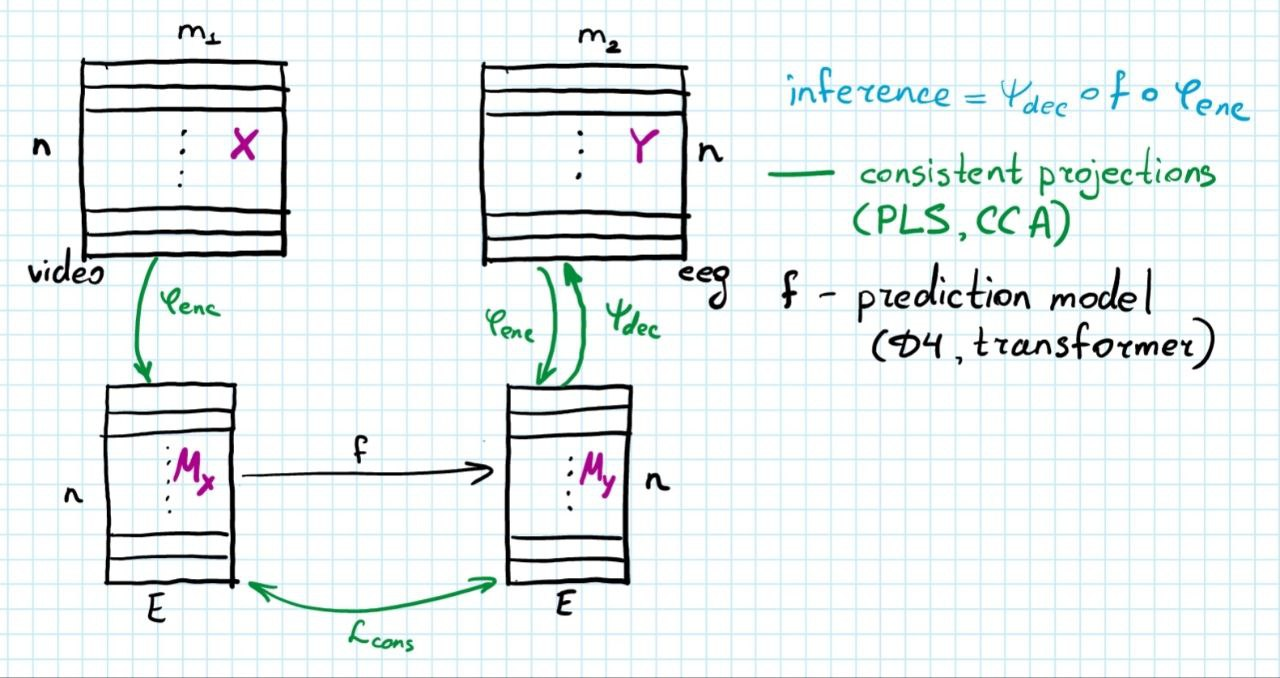
\includegraphics[width=\linewidth]{problem.jpg}

\subsection{Модель D4}
TODO

%%%%%%%%%%%%%%%%%%%%%%%%%%%%%%%%%%%%%%%%%%%%%%%%%%%%%%%%%%%%%%%%%%%%%%%%%%%%%%%%%%%%%%%%%%%%%%%%%%%%%%%%%%%%%%%%%%%%%%%%%%%%%%%%%%%%%%%
\section{Обзор литературы}
TODO

%%%%%%%%%%%%%%%%%%%%%%%%%%%%%%%%%%%%%%%%%%%%%%%%%%%%%%%%%%%%%%%%%%%%%%%%%%%%%%%%%%%%%%%%%%%%%%%%%%%%%%%%%%%%%%%%%%%%%%%%%%%%%%%%%%%%%%%
\section{Модели пространства состояний}

%%%%%%%%%%%%%%%%%%%%%%%%%%%%%%%%%%%%%%%%%%%%%%%%%%%%%%%%%%%%%%%%%%%%%%%%%%%%%%%%%%%%%%%%%%%%%%%%%%%%%%%%%%%%%%%%%%%%%%%%%%%%%%%%
\section{Вычислительный эксперимент}
Целью эксперимента является TODO.

\subsection{Экспериментальные данные}
TODO

\subsection{Условия проведения эксперимента}
TODO

\subsection{Анализ ошибки}
TODO


%%%%%%%%%%%%%%%%%%%%%%%%%%%%%%%%%%%%%%%%%%%%%%%%%%%%%%%%%%%%%%%%%%%%%%%%%%%%%%%%%%%%%%%%%%%%%%%%%%%%%%%%%%%%%%%%%%%%%%%%%%%%%%%%%%%%%%%
\section{Заключение}
TODO.

%%%%%%%%%%%%%%%%%%%%%%%%%%%%%%%%%%%%%%%%%%%%%%%%%%%%%%%%%%%%%%%%%%%%%%%%%
\addcontentsline{toc}{section}{\protect\numberline{}Список литературы}
\bibliographystyle{unsrtnat}
\bibliography{references.bib}

\end{document} 